\documentclass{article}

% Language setting
% Replace `english' with e.g. `spanish' to change the document language
\usepackage[english]{babel}

% Set page size and margins
% Replace `letterpaper' with`a4paper' for UK/EU standard size
\usepackage[letterpaper,top=2cm,bottom=2cm,left=3cm,right=3cm,marginparwidth=1.75cm]{geometry}

% Useful packages
\usepackage{amsmath}
\usepackage{graphicx}
\usepackage[colorlinks=true, allcolors=blue]{hyperref}

\title{Comparing Regression, Autoencoder and Generative
Adversarial Network (GAN) for Image Colorization}
\author{Vikram Bharadwaj, Sudhanva Narayana \\ 
        CS6140 Machine Learning \\
        Professor: Dr. Ehsan Elhamifar \\}
\begin{document}
\maketitle

%----------------------------- Abstract -----------------------------%
\begin{abstract}
Traditional image colorization methods are based on manual colorization methods such as Photoshop or GIMP.
However, these methods are not robust to the changes in the lighting conditions of the scene.
Recent advances in deep learning have made it possible to learn a colorization model from grayscale images, where the input for the networks are a set of grayscale images and the output the network learns is the colorized image. 
In this work, we present three methods for colorization: regression, autoencoder and generative adversarial network (GAN).
\end{abstract}

%----------------------------- Introduction -----------------------------%
\section{Introduction}
Every color image is a combination of 3 channels, namely: R, G, and B. 
Another way used to represent images is called the L, *a, *b (CIELAB) colorspace.
The idea is to use grayscale images for complex image processing. 
The goal of this study is to develop a method for colorizing grayscale images using the three aforementioned methods:

- \textbf{Convolutional Neural Network + Regression:} Loss between actual values of *a and *b channels and predicted *a and *b channels using vanilla CNN, followed by regression.

- \textbf{Convnet Autoencoder:} Uses CNN in an encoder-decoder fashion, where the encoder represents the grayscale image as a latent representation, which the decoder then converts to a 3-channel color image.

- \textbf{GAN:}  Uses a custom minimax log-loss function with a generator and a discriminator. The generator takes a grayscale image as an input, which it tries to convert to a 3-channel color image. The discriminator tries to tell 2 sets of images apart, i.e., (grayscale, original-color) and (grayscale, generator-color-image).

%----------------------------- Technical Details -----------------------------%
\section{Technical Details}
This task can be formulated as a problem of data imputation in which the color values of \textbf{*a} and \textbf{*b} values are "hallucinated".
The mapping from a grayscale channel to color channels is a non-deterministic problem. 
The range of values that each grayscale pixel can predict is exponentially large and the mapping is non-linear. 

%----------------------------- Method 1: Regression -----------------------------%
\subsection{Method 1: Regression}
We first use several convolutional layers to extract semantic information from the input images and then apply deconvolutional layers to upscale the extracted information.
Here, we are using pure upsample, where there are no parameters to be learned.
Specifically, the beginning of our model is a ResNet-18, an image classification network with 18 layers and residual connections. 
We modify the first layer of the network to accept grayscale input images and cut it off after the 6th set of layers. 
It predicts a two-element vector (AB channel) for each pixel of the image at the end of the network, as shown in the figure below.
\\
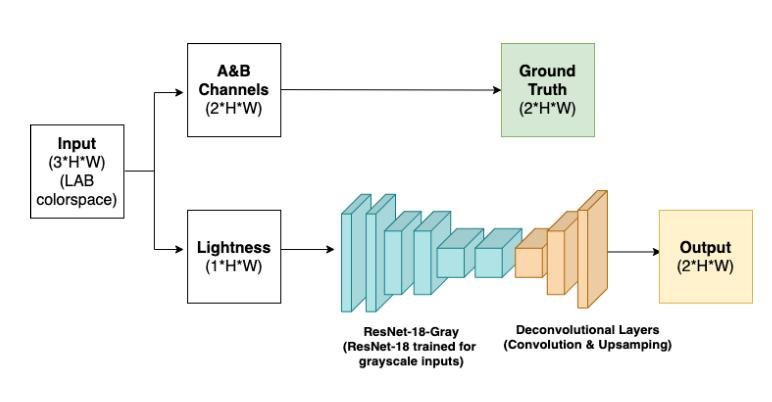
\includegraphics[width=\linewidth]{reg.jpg}

We want to minimize the Euclidean error between the AB channel we estimate and the ground truth.
However, this loss function is problematic for colorization due to the multimodality of the problem since there may be multiple plausible solutions.
As a result, our model will usually choose desaturated colors which are less likely to be correct, and the model prefers more desaturated colors than running the risk of choosing colors that are too bright.

%----------------------------- Loss Function: Regression -----------------------------%

\subsection{Loss Function: Regression}
The loss function for this problem is the Euclidean distance between the predicted AB channel and the ground truth and can be written as:
{\Large
\begin{equation}
    \ell(x,y) = \sum_{i=1}^{n} \left( x_{AB} - y_{AB} \right)^2
\end{equation}}

%----------------------------- Method 2: Autoencoder -----------------------------%

\subsection{Method 2: Autoencoder}
In this method, we use a convolutional autoencoder to learn a mapping from grayscale to color.
The encoder is a convolutional neural network, which reduces the given grayscale image to a dense latent representation, from which the decoder reconstructs the AB channels of the image.
Therefore, in this method, we have two CNNs, one for the encoder and one for the decoder.
The upsampling layers in the decoder are transposed convolutional layers, where there are a lot of parameters to be learned by the model while reconstructing the AB channels of the image.
The architecture of the entire network is as shown in the figure below.
\\
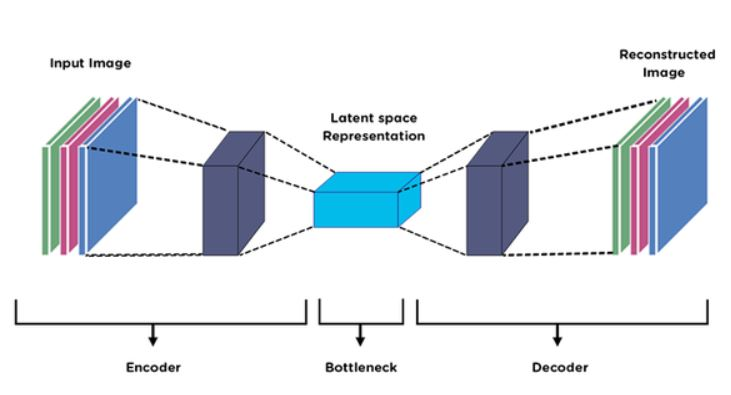
\includegraphics{autoencoder.jpg}

%----------------------------- Loss Function: Autoencoder -----------------------------%

\subsection{Loss Function}
The loss function for this method is the Euclidean distance between the predicted AB channel and the ground truth and is the same as (1).

%----------------------------- Architecture -----------------------------%

\subsection{Architecture}
\setlength{\arrayrulewidth}{0.5mm}
\setlength{\tabcolsep}{18pt}
\renewcommand{\arraystretch}{1.5}
\begin{tabular}{ |p{3cm}|p{3cm}|p{3cm}|  }
\hline
\multicolumn{3}{|c|}{Convolutional Autoencoder} \\
\hline
Encoder & Fusion & Decoder \\
\hline
Conv2D 32 x 3 x 3 - ReLu & Fusion &  \\
Aland Islands & AX   & ALA \\
Albania &AL & ALB \\
Algeria    &DZ & DZA \\
American Samoa & AS & ASM \\
Andorra & AD & AND   \\
Angola & AO & tanh \\
\hline
\end{tabular}

%----------------------------- Method 3: Generative Adversarial Network -----------------------------%

\subsection{Method 3: Generative Adversarial Network}
Unlike the previous two models, this model contains two neural networks: a generator and a discriminator. 
The generator works like previous models, takes in a black-white image and outputs the predicted colored image.
The discriminator is trained on two sets of images, to classify the predicted color image as false and the ground-truth color image as true. 
The pipeline of the model on a black-white image and the corresponding colored image is shown in the figure below.

In terms of loss function, there are two main loss functions applied here. 
First, the loss of the discriminator is computed as the average of its loss on a true image and its loss on a fake image. 
Each loss is a MSE loss for each pixel on the image (labeled 0 or 1). 
This loss could effectively capture whether this discriminator could distinguish between ground-truth image and generated image.
Second, the loss of the generator is $\lambda$ times L1 loss between predicted image and true image, plus discriminator loss on predicted image with label true.
This loss could make the generator generate images that have less difference with true image and less loss from the discriminator.


%----------------------------- Loss Function: GAN -----------------------------%
\subsection{Loss Function}
The loss function in a GAN is the following:
\begin{equation}
    \ell(x,y) = \frac{1}{2} \left( \sum_{i=1}^{n} \left( x_{AB} - y_{AB} \right)^2 + \lambda \sum_{i=1}^{n} \left( x_{AB} - y_{AB} \right)^2 \right)
\end{equation}
% $$\min_{G}\max_{D}\mathbb{E}_{x\sim p_{\text{data}}(x)}[\log{D(x)}] +  \mathbb{E}_{z\sim p_{\text{z}}(z)}[1 - \log{D(G(z))}]$$
% \begin{center}
    % 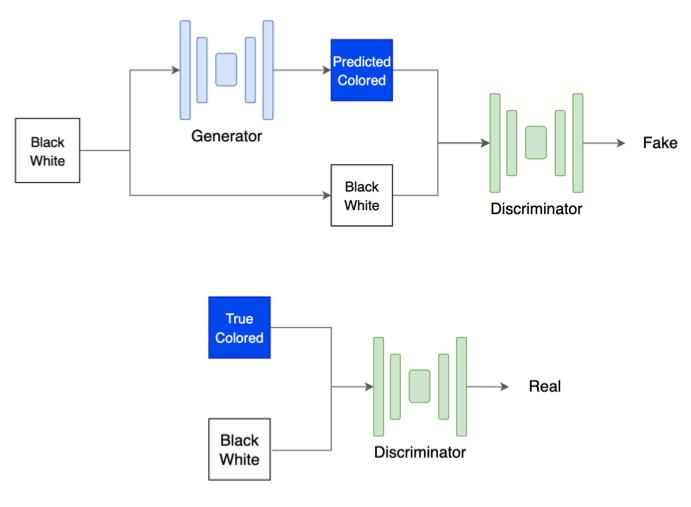
\includegraphics[width=15cm, height=10cm]{gan.jpg}
% \end{center}


%----------------------------- Experimental Results -----------------------------%
\section{Experimental Results}


%----------------------------- Dataset -----------------------------%
\subsection{Dataset}
Our training, validation and test datasets are picked from the validation set pof MIT's Places 365 \cite{7}. The dataset is from the CSAILVision Lab and can be accessed at \url{places2.csail.mit.edu/}.
All the images are in RGB format, and are 256x256 pixels in size. All channel values are in the range [0, 255].
Since there are more than 30,000 images, due to time and compute constraints, we only use a subset of the dataset of around 2,500 images for training and an additional 500 images for validation.

%----------------------------- Preprocessing -----------------------------%
\subsection{Preprocessing}
To reduce the complexity of the entire process, we use grayscale images by first converting the RGB imagesto the L*a*b color space.
The L channel is the grayscale image, and the a and b channels are the color channels.
Our models are now trained on this L channel to predict the values of the a and b channels.

%----------------------------- Pre-processing for Regression and Autoencoder -----------------------------%
\subsubsection{Pre-processing for Regression and Autoencoder}
    - All images are first converted to L*a*b channel image from RGB channel. \\
    - The L channel first extracted from the L*a*b channel image and this serves as the input to the regression model. \\
    - The *a and *b channels are used as the tragets for the regression model. \\
    - The images are then resized to a fixed size of 224x224. \\
    - The images are then normalized in the range of [-1, 1] for *a and *b channels. \\
    - The training set is then used to train the model. \\

%----------------------------- Pre-processing for Convnet based encoder-decoder and GAN -----------------------------%   
\subsubsection{Pre-processing for Convnet based encoder-decoder and GAN}
Here, we will use the same pre-processing steps as for the regression method. 
The only difference is that we will use a CNN in an encoder-decoder fashion for the second method and a GAN for the third, as shown below:

%----------------------------- Implementation -----------------------------%
\subsection{Implementation}
The idea is to use grayscale images for complex image processing. 
The goal of this study is to develop a method for colorizing grayscale images using Regression and
compare how the model performs against the use of an autoencoder and a GAN. 

%----------------------------- Results -----------------------------%
\subsection{Results}
The idea is to use grayscale images for complex image processing. The goal of this
study is to develop a method for colorizing grayscale images using Regression and
compare how the model performs against the use of an autoencoder and a GAN. 

%----------------------------- Limitations and Further Work -----------------------------%
\section{Limitations and Further Work}
The idea is to use grayscale images for complex image processing. The goal of this
study is to develop a method for colorizing grayscale images using Regression and
compare how the model performs against the use of an autoencoder and a GAN. 

%----------------------------- Contribution -----------------------------%
\section{Contribution}

The code and instructions to use or run it are available at \url{github.com/nsudhanva/image-colorization}. 
The project was built with both Vikram and Sudhanva as collaborators in the same repository with each of them being collaborative on code, reports and training.

\

\textbf{Sudhanva Narayana} implemented:
\begin{itemize}
\item GAN architecture, code, tests and experiments.
\item Trained the models on the dataset on AWS/Colab/GPU.
\item Model inferencing and reporting.
\end{itemize}



\textbf{Vikram Bharadwaj} implemented:
\begin{itemize}
\item Regression architecture, code, tests and experiments.
\item Autoencoder architecture, code, tests and experiments.
\item Model turning and reporting.
\end{itemize}

\cite{1}
\cite{2}
\cite{4}
\cite{5}
\cite{6}
\cite{7}
\cite{8}
\bibliographystyle{plain}
\bibliography{sample}

\end{document}